\chapter{Introduction}
% 1-3 pages
% It's a good idea to try to write the introduction to your final report early on in the project. 
% However, you will find it hard, as you won’t yet have a complete story and you won’t know what your main contributions are going to be. 
% However, the exercise is useful as it will tell you what you don’t yet know and thus what questions your project should aim to answer. 
% For the interim report this section should be a short, succinct, summary of the project’s main objectives. 
% Some of this material may be re-usable in your final report, but the chances are that your final introduction will be quite different.  
% You are therefore advised to keep this part of the interim report short, focusing on the following questions: What is the problem, why is it interesting and what’s your main idea for solving it?  
% (DON'T use those three questions as subheadings however!  The answers should emerge from what you write.)
There has been a particular interest in the use of drones (UAVs) for various applications, especially in areas of data collection which are traditionally difficult to access~\cite{droneReview}.
In a dense forest environment, drones have the ability to navigate faster with less disturbance to the environment.
This can allow for very efficient data collection for a variety of tasks \cite{environmentalSensing} such as autonomous sensor placement, wherein a sensor is placed in a forest environment for a long period of time.

One of the major limitations of the widespread adoption of UAVs for long-term environmental sensing is their limited flight time.
This is constrained by their limited battery capacity and the power required to sustain flight~\cite{droneBattery}.
Increasing battery capacity leads to an increase in weight carried by the drone which in turn reduces the flight time.
Current strategies to extend the flight time include improving battery technology to increase battery capacity with the same weight and incorporating solar cells into UAVs to allow for the capture of energy during flight \cite{droneSunlight}.
However, this approach relies on good environmental conditions which are difficult due to the absence of light in dense forest environments.

Alternatively to increasing battery capacity, the power required can be reduced.
However, this approach is still limited due to the theoretical minimum energy required to provide lift, which is required to keep the drone in the air.
Another approach would be to not keep the drone in the air at all.
This effectively pauses the drone which removes the main source of energy usage.
This could be achieved by landing the drone and allowing it to carry out environmental sensing from the ground.
However this leaves the UAV susceptible to damage from unsafe landing spots or animals, additionally, this is more likely to disturb the environment, reducing the validity of the results.

Taking inspiration from birds in nature another approach would be perching the UAV upon a branch which would allow for effective sensing of environments while reducing the impact on results and protecting the drone.
This approach also allows for silent operation allowing the observation of wildlife.
The majority of the current literature focuses on mechanical attachment methods.
This project aims to generate agile trajectories for tethered drone perching, effectively automating the process.

\todo{make this figure better with l, w}

\begin{figure}[htbp]
  \centering
  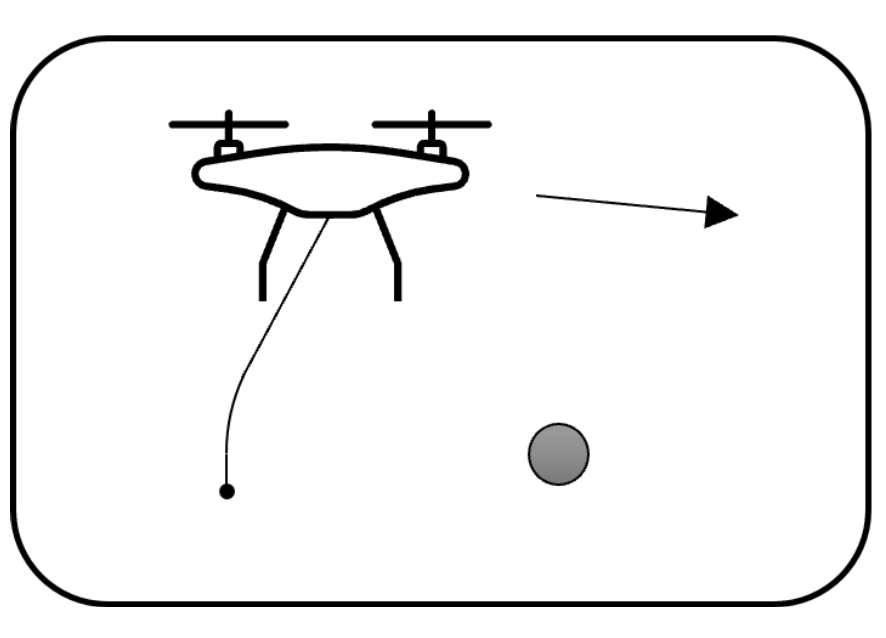
\includegraphics[width=0.33\textwidth]{introduction/tetheredDroneImage.png}
  \caption{Tethered Drone: A UAV with a tether attached with a small weight}
\label{fig:intro-tethered-drone}
\end{figure}

A tethered drone employs a pendulum mechanism, including a rope of length with a weight at one end, allowing the pendulum to move freely as shown in Figure.~\ref*{fig:intro-tethered-drone}.
For perching on a tree, the drone's tether system is designed to wrap around a target branch as shown in Figure.~\ref{fig:intro-wrapping}.
This process is further explained in Section 2.1.

\todo{improve this figure to actually show the landing}
\begin{figure}[htbp]
  \centering
  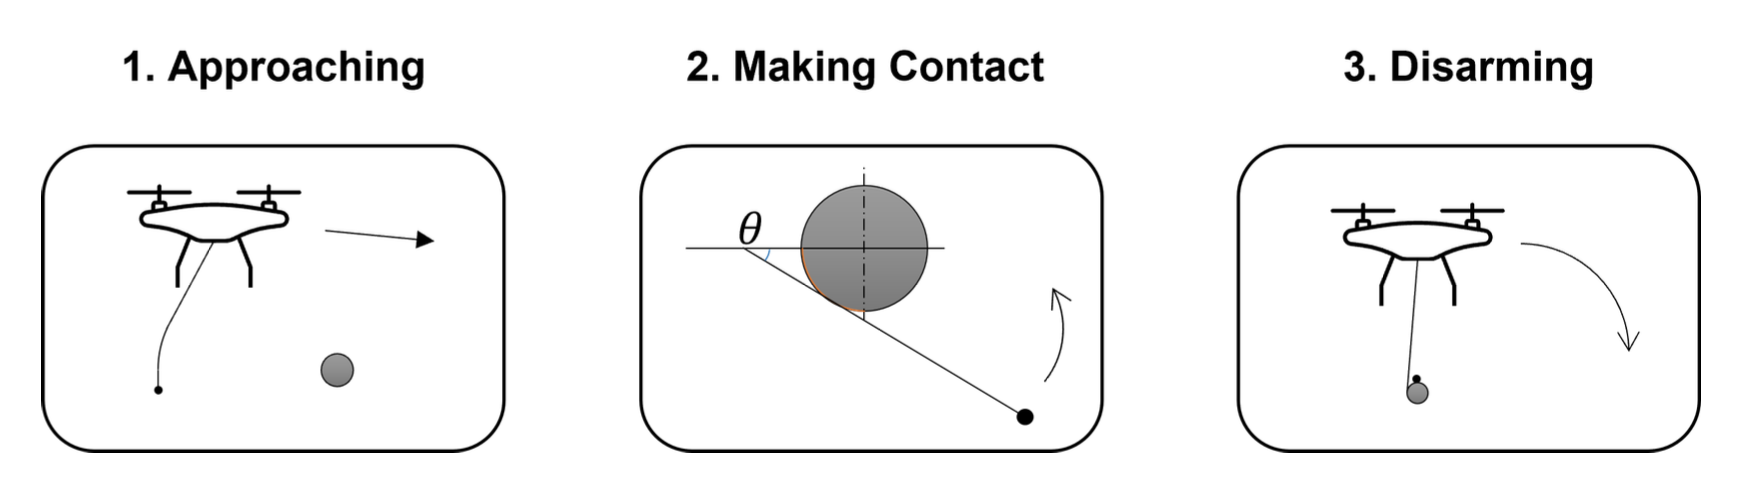
\includegraphics[width=\textwidth]{introduction/dronePerching.png}
  \caption{The 3-step process showing the drone attaching to a branch.}
\label{fig:intro-wrapping}
\end{figure}

One of the major challenges encountered in previous work in the area was in simulation.
It was difficult to simulate the pendulum and all of the forces exerted on it.
Additionally modelling the tether wrapping around the branch proved to be extremely difficult.
Therefore several assumptions had to be made that didn't necessarily prove to be correct when done on real data.
In some sections, the simulations were done without the tether being present, it was noted that this seemed oversimplified and caused trajectories to be generated that were infeasible.
This therefore motivates the need for an algorithm that can learn from real-world non-simulated environments quickly and safely.

In previous work, a demonstration, target trajectory, was used to speed up training.
However the major issue is that the reinforcement learning agent is limited to the ability of the demonstration, it assumes the demonstration is perfect which is usually not the case.
This motivates the learning of trajectories from non-expert demonstrations.
This project aims to design and implement a framework for learning agile perching trajectories from non-expert demonstrations.
This work therefore fits into the intersection between Imitation Learning (IR) and Reinforcement Learning (RL).